\chapter{Grundlagen der Signalverarbeitung}

Ein \emph{Signal} ist eine Funktion eines Parameters mit numerischen Wertebereich. Die Abbildung zwischen Defintions- und Wertebereich kann, aber muss nicht durch eine Formel definiert sein. So fällt $f(x) = \sin( x )$ genauso unter die Definition eines Signals wie eine Folge numerischer Werte, die durch die Aufnahme eines Messgerätes enstanden sind. Weiterhin kommt dem Wertebereich eine gewissen Bedeutung zu, wie \emph{Zeit} oder \emph{Ort}. Ein typisches Beispiel für ein Signal ist die Spannung, die abhängig von der Zeit von einem Mikrofon erzeugt wird.  Da in dieser Arbeit nur Signale von Bedeutung sind, deren Wertebereich sich auf die Zeit bezieht, konzetrieren sich alle folgenden Bereich auf diesen Bereich- Im Zusammenhang mit Signalen wird der Definitionsbereich auch als \emph{unabhängiger Parameter} und der Wertebereich auch als \emph{abhängiger Parameter} bezeichnet. \cite[S. 11-12]{dspGuide} \cite[S. 22-23]{dspMichigan}

%\emph{ } 
\medskip

 Bei einem zeit-kontinuierlichen Signal $x( t )$ ist der Wertebereich kontinuierlich, wie in Formel  \ref{eq:time-cont-signal} definiert. Bei einem zeit-diskreten Signal $x[n]$ ist der Wertebreich diskret, wie in Formel \ref{eq:time-disc-signal} definiert. So beschreibt beispielsweise $x[17] = s$ den Wert zur Zeit $n = 17$. \glqq Zeit\grqq{} hat in diesem Kontext keine Einheit. Ein Wert wird auch als \emph{Sample} oder \emph{Amplitude} bezeichnet. $x[17] $ meint somit das 17. Sample des Signals. Abbildung \ref{img:aSignal} zeigt Beispiele für ein zeit-kontinuierliches und ein zeit-diskretes Signal. \cite[S. 22 - 23]{dspMichigan}

 \begin{equation}
x(t) = s \; , t \in \mathbb{R}
\label{eq:time-cont-signal}
\end{equation}


\begin{equation}
x[n] = s \; , n \in \mathbb{Z} 
\label{eq:time-disc-signal}
\end{equation}

\begin{figure}
	\centering
	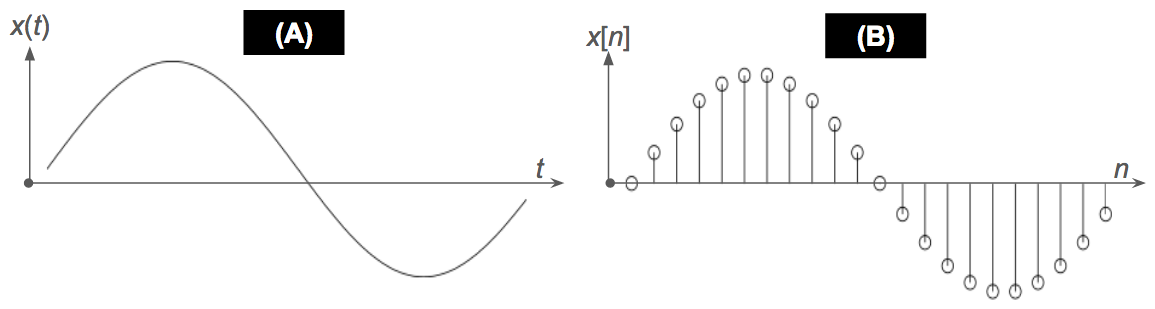
\includegraphics[width=0.7\textwidth]{bilder/aSignal02.png}
	\caption{Ein zeit-kontinuierliches Signal (A) und ein zeit-diskretes Signal (B)}
	\label{img:aSignal}
\end{figure}

Zeit-diskrete Signale werden häufig dadurch gewonnen, dass ein zeit-kontinuierliches Signal in regelmäßigen Intervallen abgetastet wird. Dieser Prozess wird als \emph{Sampling} bezeichnet und durch Formel \ref{eq:sampling} definiert. Der Parameter $T_s$ wird als \emph{Sampling-Interval} bezeichnet. Das Reziproke des Sampling-Intervals heißt \emph{Sampling-Rate} und wird in der Einheit $\frac{1}{\text{s}} = \text{Hz}$, siehe Formel \ref{eq:samplingRate}. Eine Sampling-Rate von $f_s = \SI{44100}{\hertz}$ bedeutete beispielsweise, dass ein Signal 44100 mal pro Sekunde abgetastet wurde.\cite[S. 24]{dspMichigan}

\begin{equation}
x[n] = s(n \cdot T_s) \; , -\infty < n < \infty
\label{eq:sampling}
\end{equation}
	
\begin{equation}
	\text{Samplingrate:} \quad f_s = \frac{1}{T_s} [\text{Hz}]
	\label{eq:samplingRate}
\end{equation}	

Das so genannte \emph{Nyquist-Shannon-Abtasttheorem} nach Formel \ref{eq:shannonTheorem} besagt, dass die Samplingrate mindestens doppelt so hoch sein muss wie die höchste im abgetasteten Signal enthaltene Frequenz. Das bedeutet im Umkehrschluss, dass die höchste im abgetasteten Signal enthaltene Frequenz die Hälfte der Abtastfrequenz entspricht.

\begin{equation}
f_s > 2 \cdot f_{max}
\label{eq:shannonTheorem}
\end{equation}	
	
Da in dieser Arbeit nur zeit-diskrete Signale von Interesse sind, werden ab diesem Punkt die Definitonen für zeit-kontinuierliche Signale ausgelassen. Der \emph{Support} ist das kleinst mögliche Zeitintervall, der alle Samples enthält, die nicht den Wert 0 haben, wie Formel \ref{eq:support} definiert. Die \emph{Dauer} eines Signales ist die Länge des Supportes nach Formel \ref{eq:duration}. Das Signal $x[n] = \cos(n) \: ,0\leq n \leq 3$ hat beispielsweise den Support $[0,3] = \{0,1,2,3\} $ und die Dauer $4$. Ein \emph{unendliches Signal} hat einen unendlichen langen Support, das heißt es gilt Duration$(x) = \infty$. Ein \emph{endliches Signal} hat einen endlichen Support, das heißt Duration$(x) \neq\infty$. Unabhängig von der Endlichkeit oder Unendlichkeit des Supportes wird davon ausgegangen, dass sich alle Signale von negativer bis positiver Unendlichkeit erstrecken. Werden also berechnungen auf Samples eines Signales durchgeführt, die außerhalb seines Supportes liegen, werden diese Samples mit dem Wert 0 angenommen. \cite[S. 24]{dspMichigan}

\begin{equation}
\label{eq:support}
\begin{split}
\text{Sup}(x) = [sup_s, sup_e] \quad , sup_s, sup_e \in \mathbb{Z} \\,  x[sup_s] \neq 0 \:  \wedge \:  x[sup_e] \neq 0 \: \wedge \: \forall n \
\not\in [sup_s, sup_e] : x[n] = 0
\end{split}
\end{equation}

\begin{equation}
\text{Duration}(x) = sup_e - sup_s + 1
\label{eq:duration}
\end{equation}

Ein Signal gilt als \emph{periodisch}, wenn Formel \ref{eq:periodicity} erfüllt ist. Der Parameter $N$ wird als \text{Periode} von $x$ bezeichnet. Wenn ein Signal mit $N$ periodisch ist, dann ist es auch mit $2N, 3N, \ldots $ periodisch. Die Grundfrequenz $N_0$ ist das kleinste N, für das Formel \ref{eq:periodicity} erfüllt ist. Abbildung \ref{img:periodicSic} zeigt ein Beispiel für ein nicht-periodisches und ein periodisches Signal. \cite[S. 24]{dspMichigan}

\begin{equation}
\exists N : \forall n \in Sup : x[n+N] = x[n] \rightarrow \text{Periodisch}(x) = true
\label{eq:periodicity}
\end{equation}

\begin{figure}[h]
	\centering
	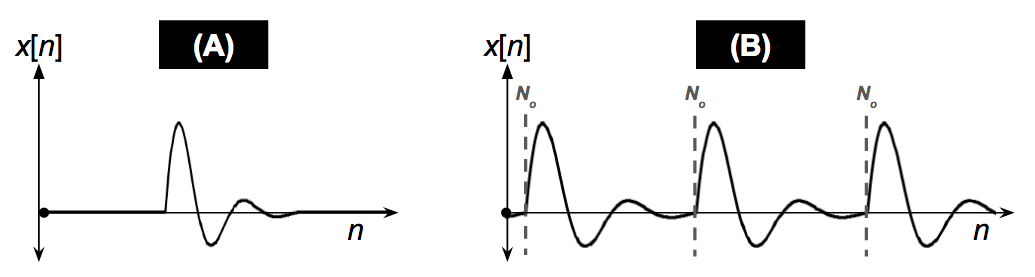
\includegraphics[width=0.7\textwidth]{bilder/periodicSig.png}
	\caption{Ein nicht-periodisches Signal (A) und ein periodisches Signal (B)}
	\label{img:periodicSic}
\end{figure}

\section{Statistische Merkmale}

Im folgenden wird ein überblick über die häufig verwendete Signaleigenschaften gegeben. Abbildung \ref{img:sigStats} visualisiert die Erläuterungen.

\begin{enumerate}[leftmargin=*]
	
\item Der \textbf{Maximalwert / Minimalwert} beschreibt den höchsten / niedrigsten in  $x$ enthaltenen Wert nach den Formel $\max(x)$ und $\min(x)$.
	
\item Der \textbf{Durchschnittswert / Average Value} beschreibt den durchschnittlichen Wert aller Samples von $x$ nach Formel \ref{eq:avg}. Dieser Durchschnittswert wird über dem Intervall $[n_1, n_2]$  berechnet.

\begin{equation}
\text{AVG}(x) = \frac{1}{n_2 - n_1 + 1} \sum_{n = n_1}^{n_2} x[n]
\label{eq:avg}
\end{equation}

\item Der \textbf{Mean Squared Value} (\emph{MSV}) beschreibt den quadrierten Durchschnittswert über eine bestimmtes Interval nach Formel \ref{eq:msv}. Er wird auch als \emph{durchschnittliche Energie} oder \emph{average Power} bezeichnet.

\begin{equation}
\text{MSV}(x) = \frac{1}{n_2 - n_1 + 1} \sum_{n = n_1}^{n_2} x[n]^2
\label{eq:msv}
\end{equation}

\item Das \textbf{Root Mean Square} (\emph{RMS}) ist die Wurzel des Mean Squared Value nach Formel\ref{eq:rms}. Der RMS findet häufiger Anwendung als der MSV, da er besser ins Verhältnis zu den Werten des Signals gesetzt werden kann. Er wird im Deutschen auch als \textbf{Effektivwert} oder \textbf{Durchschnittsleistung} bezeichnet. Da die deutschen Begriffe in einigen Quellen jedoch auch für den MSV verwendet werden, wird an dieser Stelle nur mit den englischen Begriffen gearbeitet.

\begin{equation}
\text{RMS}(x) = \sqrt{\frac{1}{n_2 - n_1 + 1} \sum_{n = n_1}^{n_2} x[n]^2}
\label{eq:rms}
\end{equation}

\item Die \textbf{Energie / Energy} bezeichnet die \glqq Stärke \grqq{} eines Signals über einen bestimmten Intervall nach Formel \ref{eq:energy}. Sie entspricht dem MSV-Wert multipliziert der Länge des Intervalls. \cite[S. 27-28]{dspMichigan}

\begin{equation}
\text{E}(x) = \sum_{n = n_1}^{n_2} x[n]^2
\label{eq:energy}
\end{equation}
	
\end{enumerate}	

\begin{figure}[h]
	\centering
	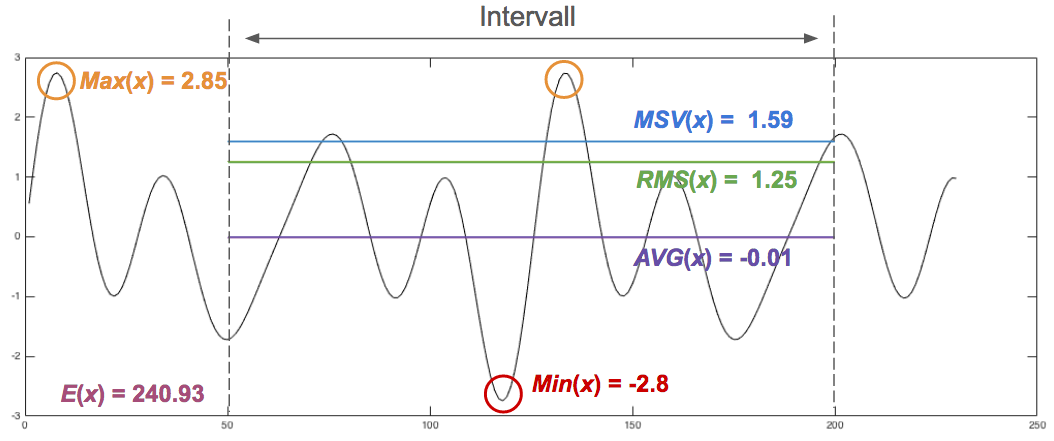
\includegraphics[width=0.7\textwidth]{bilder/sigStats.png}
	\caption{Statistische Werte eines Signals über das Intervall [50,200]}
	\label{img:sigStats}
\end{figure}

Die Addition und Multiplikation wird bei Signalen komponentenweise durchgeführt, das heißt $x_1[n] + x_2[n] = y[n] $ und $x_1[n] \cdot x_2[n] = y[n] $. Abbildung \ref{img:addAndMultSig} visualisiert diese Operationen. 

\begin{figure}[h]
	\centering
	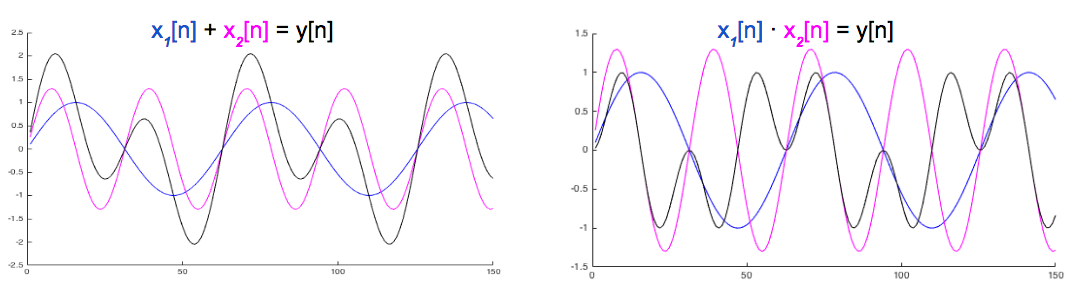
\includegraphics[width=0.8\textwidth]{bilder/addAndMultSig.png}
	\caption{Komponentenweise Addition und Mulitplikation zweier Signale}
	\label{img:addAndMultSig}
\end{figure}

\section{Fehlersignale}

Die Addition wird unter anderem für die Modellierung des Einflusses von Störungen benötigt. Angenommen, ein Signal $x$ wird übertragen, auf dem Übertragungsweg jedoch durch ein anderes Störsignal wie z.B. Rauschen $e$ überlagert. Dieses Störsignal wird in diesem Zusammenhang auch als \glqq{Fehler-Signal} bezeichnet. Das resultierende Signal $x'$ wird nach Formel \ref{eq:sigErrorAddition} berechnet. Kennt man sowohl das Eingangssignal $x$ als auch das Ausgangssignal $x'$, kann das Störsignal $e$ nach Formel \ref{eq:calErrorSig} berechnet werden.

\begin{equation}
x'[n] = x[n] + e[n]
\label{eq:sigErrorAddition}
\end{equation}

\begin{equation}
e[n] = x'[n] -x[n]
\label{eq:calErrorSig}
\end{equation}

 Errechnet man nun den den MSV- oder RMS-Wert des Störsignales $e$, gibt das Ergebnis einen Eindrück über die \glqq Stärke \grqq{} des Fehler-Signals. Der MSE-Wert des Fehlers wird in diesem Zusammenhang auch als \emph{Mean Squared Error} (\emph{MSE}) und der RMS-Wert als \emph{Root Mean Squared Error} (\emph{RMSE}) oder einfach als \emph{Fehler} oder \emph{Error} bezeichnet. Formel\ref{eq:mse} und \ref{eq:error} definierten die Berechnungen des MSE und RMSE. Der RMSE hat im Gegensatz zum MSE den Vorteil, dass er besser ins Verhältnis zu den Werten des Fehlersignals gestetzt werden kann. Ein RMSE $= 0$ heisst, dass $x = x'$ und somit kein Störsignal vorliegt. Ein RMSE = RMS$(x)$ heisst, dass Eingangs- und Störsignal den selben Effektivwert und somit die selbe \glqq stärke\grqq{} besitzen. Abbildung \ref{img:snrStuff} visualisiert die Berechnung des MSE und RMSE. \cite[S: 28 - 29]{dspMichigan}

\begin{equation}
\text{MSE}(x,x') = \frac{1}{n_2 - n_1 + 1} \sum_{n = n_1}^{n_2} (x[n]-x'[n])^2
\label{eq:mse}
\end{equation}

\begin{equation}
\text{RMSE}(x,x') = \sqrt{\frac{1}{n_2 - n_1 + 1} \sum_{n = n_1}^{n_2} (x[n]-x'[n])^2}
\label{eq:error}
\end{equation}

Eine weitere Betrachtungsweise bezüglich der Stärke des Rauschens auf das Signal ist, das Eingangssignal ins Verhältnis zum Rauschsignal zu setzen. Formel \ref{eq:snrPre} gibt die Definition. Ein SNR\textsubscript{rel}$(x,e) = 1$ heißt, dass das Eingangssignal den selben MSV wie das Fehlersignal hat. Meistens ist der MSV des Eingangssignals in der Praxis sehr viel höher als der des Fehler-Signals. Um den Zahlenraum zu begrenzen, wird die Pseudo-Einheit dB verwendet. Formel \ref{eq:snrDb} den so berechneten \emph{Signal-Rausch-Abstand} (\emph{SNR}, englisch Signal-to-Noise-Ratio). Entgegen des MSE weisst ein \emph{niedriger} SNR-Wert auf ein \emph{starkes} Rauschen hin, und ein \emph{hoher} SNR auf ein \emph{schwaches} Rauschen! Abbildung \ref{img:snrStuff} visualisiert die Berechnung des SNR.

%% To do: Gute Quelle suchen!!

\begin{equation}
\text{SNR}_{rel}(x,e) = \frac{MSV(x)}{MSV(e)}
\label{eq:snrPre}
\end{equation}

\begin{equation}
\text{SNR}(x,e) = 10 \cdot  \lg \Big(\frac{MSV(x)}{MSV(e)} \Big) \text{ dB}
\label{eq:snrDb}
\end{equation}

\begin{figure}[h]
	\centering
	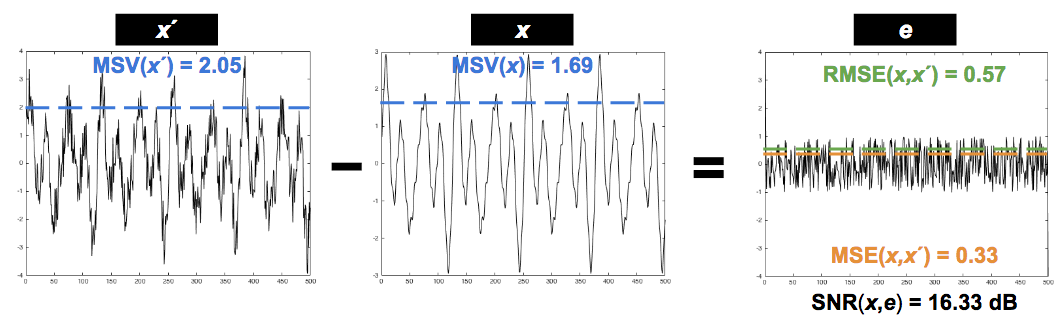
\includegraphics[width=1\textwidth]{bilder/snrStuff02.png}
	\caption{Berechnung des MSE, RMSE und SNR eines von Rauschen gestörten Signals}
	\label{img:snrStuff}
\end{figure}

\section{Korrelation}
\label{sec:correlation}

Die \emph{Korrelation} (engl \emph{Correlation}) zweier Signale $x_1$ und $x_2$ wird nach Formel \ref{eq:correlation} als die Summe aller Samples des Produktes der beiden Signale über einen bestimmtes Intervall $[n_1, n_2]$ definiert. Das Ergebnis ist eine Wert $\in \mathbb{R}$ welches die \glqq Ähnlichkeit der beiden Signale\grqq{} kennzeichnet. Ein Positiver Wert weisst auf eine \emph{positive Korrelation} hin, ein negativer Wert auf eine \emph{negative Korrelation}, und ein Wert von $\text{Corr}(x_1,x_2) = 0$ auf \emph{keine Korrelatoin}. Aus der größe des Wertes kann die Stärke der Korrelation jedoch nicht direkt interpretiert werden. Bei der \emph{normalisierten Korrelation} Corr$_N(x,y)$ wird daher die Korrelationswert ins Verhältnis zu den Energien der beiden Signale gesetzt, wie in Formel \ref{eq:normCorrelation} definiert. Der Wertebereich der normalisierten Autokorrelation  ist $-1 \leq \text{Corr}_N(x,y) \leq +1$. Daraus ergeben sich die in Formel \ref{eq:correlationProps} definierten Zusammenhänge. Ein Wert von $ \text{Corr}_N(x,y) = 1$ wird auch als \emph{perfekte Korrelation} bezeichnet, ein Wert von  $ \text{Corr}_N(x,y) = -1$ als \emph{anti-perfekte Korrelation} \cite[S. 46 - 47]{dspMichigan} Abbildung \ref{img:corrSigsComp} visualisiert die normalisierte Korrelation eines Signales $x$ mit den Signalen $y_n$.

\begin{equation}
\text{Corr}(x,y) = \sum_{n=n_1}^{n_2} x[n] \cdot y[n]
\label{eq:correlation}
\end{equation}

\begin{equation}
\text{Corr}_N(x,y) = \frac{\text{Corr}(x,y)}{\sqrt{\text{E}(x) \cdot \text{E}(y)}}
\label{eq:normCorrelation}
\end{equation}

\begin{equation}
\text{Corr}_N(x,y) = 
\begin{cases}
1  \quad \rightarrow  x = y \\
-1 \; \rightarrow x = -y
\end{cases}
\label{eq:correlationProps}
\end{equation}

\begin{figure}[h]
	\centering
	\includegraphics[width=1\textwidth]{bilder/corrSigsComp.png}
	\caption{Correlation der Signale $x$ und $y$}
	\label{img:corrSigsComp}
\end{figure}

Die Korrelation und die normalisierte Korrelation werden aufgrund ihrer Eigenschaften verwendet, um ein Signal $x$ in einem Signal $y$ zu detektieren. Häufig ist das Ziel, ein von einem Rauschen $e$ überlagerten Signal $x+e = y$ auf das Vorhandensein des erwarteten Signales $x$ hin zu überprüfen. Wie in Abbildung \ref{img:corrSigsComp} zu sehen ist, ist der Korrelationswert jedoch von der Verzögerung des Signals abhängig. Daher wird in der $Cross-Correlation$ das Signal $y$ mit einer verzögerten Varianten des Signals $x$ korreliert, wie in Formel \ref{eq:XCorr} definiert. Der parameter $k$ wird als \emph{Lag} bezeichnet und gibt die Verzögerung an. 

\begin{equation}
\text{X-Corr}(x,y,k) = \sum_{n=-\infty}^{\infty} x[n-k] \cdot y[n]
\label{eq:XCorr}
\end{equation}

Im Prozess der so genannten \emph{Running Correlation} nutzt man die Cross-Correlation mit den Lags $k = 0 \cdots k_{max}$ zur Erstellung des \emph{Korrelationssignals} $r$, wie in Gleichung \ref{eq:runningCorrelation} definiert. Das Signal $r$ gibt Auskunft, zu welchen Verzögerungswerten $k$ die größten Ähnlichkeiten zwischen $x$ und $y$ gefunden wurden. 

\begin{equation}
r[k] = \text{X-Corr}(x,y,k) \quad, k = 0 , \ldots , k_{max} 
\label{eq:runningCorrelation}
\end{equation}

Abbildung \ref{img:slidingCorrelation} zeigt ein Beispiel für die Erzeugung von $r$ mit der Sliding Correlation. (A) zeigt das zu detektierende Signal $x$ und (B) das Signal $y$. (C) zeigt das Korrelationssignal $r$ mit den Lags $k = 1, \ldots ,1150$ \cite[S. 47 - 48]{dspMichigan}

\begin{figure}[h]
	\centering
	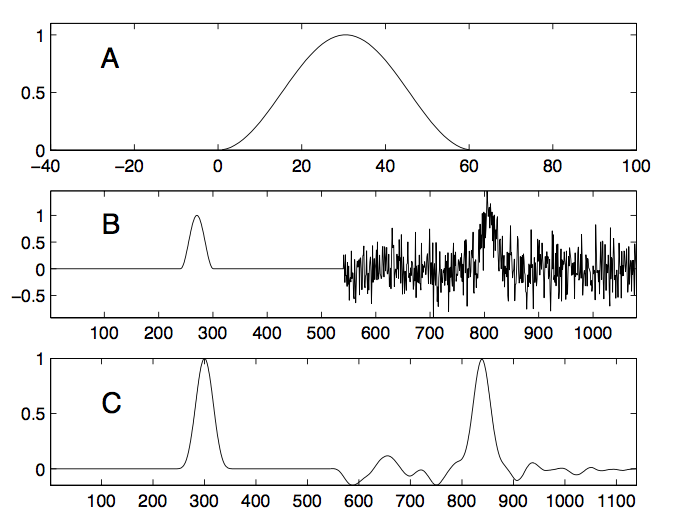
\includegraphics[width=0.5\textwidth]{bilder/slidingCorrelation.png}
	\caption{Beispiel einer Running Correlation}
	\label{img:slidingCorrelation}
\end{figure}

\section{Faltung}

Die \emph{Faltung} (engl. \emph{Convolution}) ist eine der Zentralen Operationen zwischen zwei Signalen, so wie die Addition oder die Mulitplikation. Sie wird mit dem Symbol $*$ notiert. Sie wird notiert mit $x* h = y$. 

Die Faltung basiert auf der \emph{Faltungs-Summe}, welche die Faltung zunächst Punktweise definiert. Die Gleichung wird in Formel \ref{eq:convolutionSum} abgebildet. In diesem Zusammenhang wird $x$ Eingangs- und $y$ als Ausgangs-Signal bezeichnet. Je nach Anwendungsfall bekommt $h$ den Namen \emph{Faltungs-Kernel}, \emph{Filter-Kernel} oder einfach \emph{Kernel}. \cite[S. 107-108]{dspGuide}

\begin{equation}
y[n] = x[n] * h[n] = \sum_{i=1}^{M} h[i] * x[n-i]
\label{eq:convolutionSum}
\end{equation}

Das Ergebnis einer Berechneten Faltungssumme nach \ref{eq:convolutionSum} ist ein einzelner Wert. Wird die Faltungs-Summe ähnlich der Cross-Correlation für $n = 1...N+M-1$ durchgeführt, ist das Ergebnis ein Signal. Die tatsächliche Faltung wird in Gleichung \ref{eq:convolution} definiert. $x$ ist ein Signal mit Support$(x) = [1,N]$ und Duration$(x) = N$, $h$ ist ein Signal mit Support$(x) = [1,M]$ und Duration$(h) = M$ und $y$ ist ein Signal mit Support$(y) = [1,N+M-1]$ und Duration$(y) = N+M-1$. Das heißt, dass das Eingangssignal um die Länge des Faltungskerns verlängert wird. Abbildung 	\ref{img:convolutionExample} zeigt ein Beispiel für die Faltung.\cite[S. 115-120]{dspGuide}

\begin{equation}
y = x * h = \big[ \: x[1] * h[1] , \ldots , x[N+M-1] * h[N+M-1] \: \big]
\label{eq:convolution}
\end{equation}

\begin{figure}[h]
	\centering
	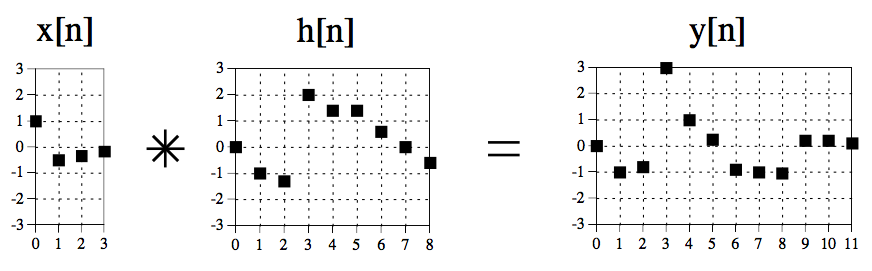
\includegraphics[width=0.7\textwidth]{bilder/convolutionExample.png}
	\caption{Beispiel für die Faltung}
	\label{img:convolutionExample}
\end{figure}

Das neutrale Element der Faltung ist der \emph{Delta-Funktion}, definiert in Gleichung \ref{eq:delta} . Das heißt, dass $x * \delta = x$ . Die Faltung ist kommutativ, das heißt $ x * h = h * x = y$ . \cite[S. 107, 113 ]{dspGuide}

\begin{equation}
\delta[n] = 
\begin{cases}
1 \quad , n = 0\\
0 \quad ,  n \neq 0
\label{eq:delta}
\end{cases}
\end{equation}

Eines der wichtigsten Anwendungsgebiete der Faltung ist das Filtern. Weitere Erläuterungen werden in Kapitel \ref{sec:filter} gegeben.


\section{Diskrete Fourier-Transformation}

Die \emph{Fourier-Transformation} ist eine Familie von Transformationen, mit deren Hilfe Signale aus dem Zeit-Bereich in den Frequenz-Bereich transformiert werden. Das heißt, dass der unabhängige Parameter nach der Transformation nicht mehr die Zeit, sondern die Frequenz beschreibt. 

Die konkrete Berechnung der Transformation ist abhängig von den Eigenschaften des Signales. Die Variante, die die meiste Anwendung in der digitalen Signalverarbeitung findet, ist die \emph{Diskrete Fourier-Transformation} (kurz \textbf{DFT} ). Sie transformiert \emph{zeit-diskrete, periodische, unendliche} Signale (siehe Formel \ref{eq:time-disc-signal} und \ref{eq:periodicity}) in den Frequenz-Bereich. Es exisitert sowohl eine reelle als auch eine complexe Variante der DFT. Die reelle Variante wird mit Hilfe reeller Zahlen, und die komplexe mit Hilfe komplexer Zahlen berechnet. An dieser Stelle werden beide Variante vorgestellt: Die komplexe, da der effizienteste Algorithmus zur Berechnung der DFT, die \emph{Fast-Fourier-Transformation} (\textbf{FFT}) auf ihr beruht, und die reelle, da sie das Verständnis der komplexen vereinfacht.\cite[S. 142 - 146]{dspGuide}

\subsection{Reelle DFT}
\label{sec:realDFT}

Jedes zeitdiskretes, periodisches Signal $x$ kann erzeugt werden, indem eine endliche Anzahl von Sinus- und Cosinus-Signalen geeigneter Frequenz und Amplitude $ = \{A_0\cos_{f_0} \ldots A_m\cos_{A_m,f_m}$ , $B_0\sin_{f_0} \ldots \sin_{f_m} \}$ aufaddiert werden. Der Umkehrschluss ist, dass sich jedes Signal in eine Menge von Sinus- und Cosinus-Signalen zerlegen lässt, ohne das Information für das Signal $x$ verloren geht. Diese Zerlegung des Signals $x$ wird als \emph{Dekomposition} bezeichnet, die Kombination der Sinus- und Cosinus-Siganel zu $x$ als \emph{Synthese}. Genauer gesagt werden für ein Signal $x$ mit Duration$(x) = N$ höchstens $\frac{N}{2}+1$ Sinus- und $\frac{N}{2}+1$ Cosinus-Wellen benötigt, also insgesamt $N+2$ Signale. Gleichung \ref{eq:fftIntroduction} fasst diese Aussage zusammen. \cite[S. 144 - 147 ]{dspGuide}

\begin{equation}
\label{eq:fftIntroduction}
\begin{split}
\forall x = [x_1 \ldots x_N]: x =  A_0\cos_{f_0} + \ldots + A_m\cos_{f_m}  + B_0\sin_{f_0} + \ldots + B_m \sin_{f_m}  \\
,\text{Periodisch}(x) = true \; ,m = \frac{N}{2}
\end{split}
\end{equation}


Die Cosinus- und Sinus-Schwingungen, die in Gleichung \ref{eq:fftIntroduction} verwendet werden, werden in den Gleichungen \ref{eq:cosine} und \ref{eq:sine} definiert, sowohl für den kontinuierlichen als auch für den zeit-diskreten-Definitionsraum. Die Faktorn $A,B$ geben die Amplitude der entsprechenden Cosinus/Sinus-Schwingung an, der Fatkor $f$ die Frequenz der Schwingung (Perioden pro Sekunde), und $f_s$ die Sampling-Rate (Siehe Gleichung \ref{eq:samplingRate}). \cite[S. 62]{dspMichigan} \cite[S. 150]{dspGuide} Abbildung \ref{img:aSimpleCosine} zeigt ein Beispiel für die Cosinus-Schwingung $[A=2] \cdot cos_{f=\SI{4}{\hertz}}$.

\begin{equation}
\label{eq:cosine}
\begin{gathered}
A \cdot \cos_{f}(t) = A \cdot \cos(2\pi f t) \\
A \cdot \cos_{f}[n]  = A \cdot \cos(2\pi f \frac{n}{f_s})
\end{gathered}
\end{equation}

\begin{equation}
\label{eq:sine}
\begin{gathered}
 B \cdot \sin_{f} (t) = B \cdot \sin(2\pi f t) \\
 B \cdot \sin_{f}[n]  = B \cdot \sin(2\pi f \frac{n}{f_s})
\end{gathered}
\end{equation}

\begin{figure}[h]
	\centering
	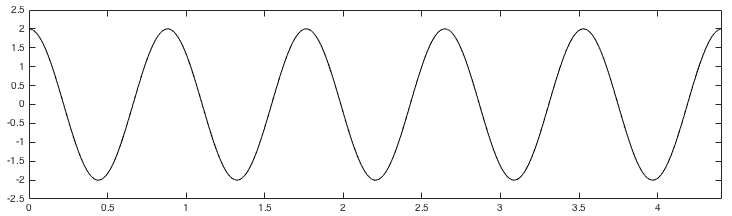
\includegraphics[width=0.7\textwidth]{bilder/aSimpleCosine.png}
	\caption{$\SI{1}{\second} = 44100 $ Samples der Cosinus-Schwingung $[A = 2] \cdot cos_{f=\SI{4}{\hertz}}[n] =  2 \cdot \cos(2\pi 4 \frac{n}{f_s})$ bei einer Sampling-Rate von $f_s = \SI{44100}{\hertz} $}
	\label{img:aSimpleCosine}
\end{figure}

Abbildung \ref{img:fftExample02} zeigt ein Beispiel für die Synthese eines Signal $x$ mit $N = 200$ Samples mit einer Samlingrate von $f_s = \SI{100}{\hertz}$. Es werden theoretisch $\frac{N}{2} + 1 = 101$ Cosinus und $101$ Sinus-Signale für die Synthese benötigt, da aber nur 4 Signale eine Amplitude > 0 haben, werden auch nur diese Signale gezeigt. Die Frage ist: Angenommen, man kennt nur das Signal $x$, wie errechnet man daraus die die Amplituden $A, B$ und Frequenzen $f$ der Cosinus- und Sinus-Signale? Anders gesagt: Wie berechnet man die Dekomposition?

\begin{figure}[h]
	\centering
	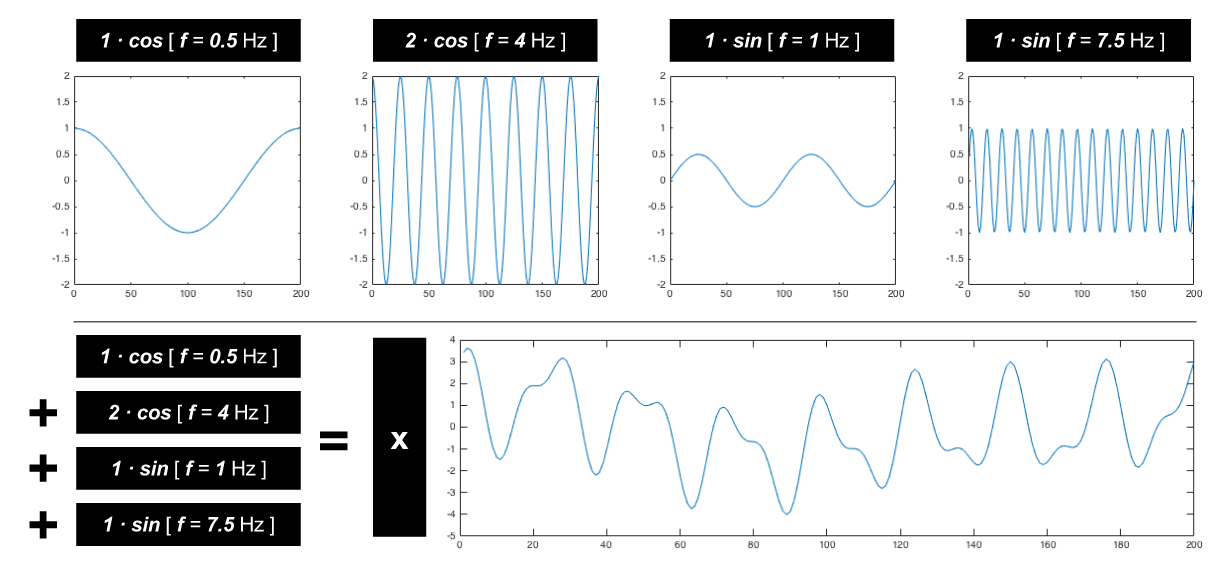
\includegraphics[width=1\textwidth]{bilder/fftExp02.png}
	\caption{Synthetisierung eines Signals $x$ aus vier Cosinus-Funktionen, mit Duration$(x) = 200$ und $f_s = \SI{100}{\hertz}$}
	\label{img:fftExample02}
\end{figure}

Das Problem lässt sich auf die Berechnung der Amplituden $A,B$ beschränken, in dem man den Fakt, dass höchstens $\frac{2}{N} + 1$ Cosinus- und $\frac{2}{N} + 1$ Sinus-Signale für die Synthese benötigt werden, in Verbindung mit dem Nyquist-Shannon-Abtasttheorem (Gleichung \ref{eq:shannonTheorem}) bringt. Die niedrigst mögliche Frequenz, die im Signal $x$ enthalten sein kann, ist $f_0 = \SI{0}{\hertz}$, und die höchst mögliche Frequenz $f_{max} = \frac{f_s}{2}$, womit die Frequenzen $\cos_{f_0 = 0} , \cos_{f_{max} = f_s/2},\sin_{f_0 = 0} , \sin_{f_{max} = f_s/2}$ bereits feststehen. Die restlichen $\frac{2}{N} - 1$ Cosinus-Signale teilen sich gleichmäßig auf diesen Frequenzraum auf, entsprechendes gilt für die Sinus-Signale. Die Frequenz der insgesamt $N+2$ Cosinus/Sinus-Signale ergibt sich somit direkt als Funktion der Samplingrate und der Länge des Signals $x$. Gleichung \ref{eq:baseFunctions} fasst diesen Zusammenhang zusammen. Die dort beschriebenen Funktionen $\cos_k$ und $\sin_k$werden als \emph{Basisfunktionen} bezeichnet. Aus dem  Index $k = 0 ... \frac{N}{2}$ lässt sich die Frequenz der jeweiligen Basisfunktion nach Gleichung \ref{eq:baseToFreq} berechnen.\cite[140 - 151, S.]{dspGuide}  In Bezug auf das Beispiel aus Abbildung \ref{img:fftExample02} ergeben sich die indexe $[\cos_{f=\SI{0.5}{\hertz}} = \cos_1]$, $[\cos_{f=\SI{4}{\hertz}} = \cos_8]$, $[\sin_{f=\SI{1}{\hertz}} = \sin_2]$ und $[\sin_{f=\SI{7.5}{\hertz}} = \sin_{15}]$

\begin{equation}
\label{eq:baseFunctions}
\begin{split}
A_k \cdot \cos_k[n] = A_k\cdot \cos(2\pi k \frac{n}{N}) \\
B_k \cdot \sin_k[n] = B_k \cdot \sin(2\pi k \frac{n}{N}) \\
N = \text{Duration} (x)
\end{split}
\end{equation} 

\begin{equation}
\label{eq:baseToFreq}
f = k\frac{f_s}{N} 
\end{equation} 

Das Problem der Dekomposition wird so auf die Suche der Amplituden-Koeffizienten $A_k, B_k$ beschränkt. Die Frage ist, vereinfacht formuliert, wie \glqq stark\grqq{} jede der Basisfunktionen $\cos_0 \ldots \cos_{N/2} , \sin_0 \ldots \sin_{N/2}$ in $x$ enthalten ist.  Die Antwort darauf ist die in Kapitel \ref{sec:correlation} vorgestellte Korrelation. Der Korrelationswert einer Cosinus-Basisfunktion mit Eingangssignal Corr$(x,\cos_k) = \sum_{n=1}^{N} \cdot x[n]cos_k$ gibt somit eine Aussage darüber, wie stark die entsprechende Cosinus-Schwingungen zur Syntehse von $x$ beiträgt. Ein Wert von $0$ spricht für keinen Beitrag, ein hoher oder niedriger Wert für eine positiven oder negativen Beitrag. \cite[S. 157 - 158]{dspGuide}

Dieses Vorgehen lässt sich sogenannten \emph{forward DFT} nach Formel \ref{eq:forwardDFT} verallgemeinern, kurz als \textbf{DFT} bezeichnet. Das Ergebnis sind die Koeffizienten $\bar{A}_0 \ldots \bar{A}_{N/2}, \bar{B}_0 \ldots \bar{B}_{N/2}$. \cite[S. 158]{dspGuide}

\begin{equation}
\begin{split}
\bar{A}_k = \sum_{n=0}^{N-1}x[n] \cos(2\pi k \frac{n}{N}) \\
\bar{B}_k = \sum_{n=0}^{N-1}x[n] \sin(2\pi k \frac{n}{N}) \\
\end{split}
\label{eq:forwardDFT}
\end{equation}

In Bezug auf das Beispiel aus Abbildung \ref{img:fftExample02} ergeben sich bei Anwendung von Formel \ref{eq:forwardDFT} auf das Signal $x$ die Koeffizienten $[ \bar{A}_{f=\SI{0.5}{\hertz}} = \bar{A}_{1} = 100 ]$ , $[  \bar{A}_{f=\SI{4}{\hertz}} = \bar{A}_{8} = 200 ]$, $[ \bar{B}_{f=\SI{1}{\hertz}} = \bar{B}_{2} = 50 ]$ und $[ \bar{B}_{f=\SI{7.5}{\hertz}} = \bar{B}_{15} = 100 ]$. Um die eigentlichen Koeffizienten $A_1 = 1, A_8 = 2, B_2 = 0.5$ und $B_{15} = 1$ zu erhalten, muss die Umrechnungsvorschrift nach den Formel \ref{eq:AConversion} und \ref{eq:BConversion} angewandt werden. \cite[S. 152 - 153]{dspGuide}

\begin{equation}
A_k = 
\begin{cases}
\frac{\bar{A}_k}{N} \; , \text{falls } k = 0 \vee k = N/2\\
\frac{\bar{A}_k}{N/2} \; ,\text{sonst} \\
\end{cases}
\label{eq:AConversion}
\end{equation}

\begin{equation}
B_k= \frac{A_k}{N/2}
\label{eq:BConversion}
\end{equation}

Gleichung \ref{eq:inverseDFT} definiert die Synthese des Signals $x$ aus den Basis-Funktionen mit Hilfe der Koeffizienten $A$ und $B$. Die Formel wird auch als \emph{inverse DFT} (\textbf{iDFT}) bezeichnet. \cite[S. 152 - 153]{dspGuide}

\begin{equation}
\begin{split}
x[n] = \sum_{k = 0}^{N/2} A_k\cos(2\pi k \frac{n}{N}) + \sum_{k = 0}^{N/2}B_k\sin(2\pi k \frac{n}{N}) \\
,n = 1 \ldots N = \text{Duration}(x)
\end{split}
\label{eq:inverseDFT}
\end{equation}

Die Koeffizienten $A$ und $B$ bilden zusammen den \emph{Frequenz-Bereich} in der sogenannten \emph{kartesischen Notation} (engl \emph{rectangular Notation}) und werden gemeinsam als $X$ bezeichnet. \cite[S. 161 - 162]{dspGuide} Abbildung  \ref{img:polarToRect02} zeigt die Koeffizienten des Beispiels aus Abbildung \ref{img:fftExample02}.


\begin{figure}[h]
	\centering
	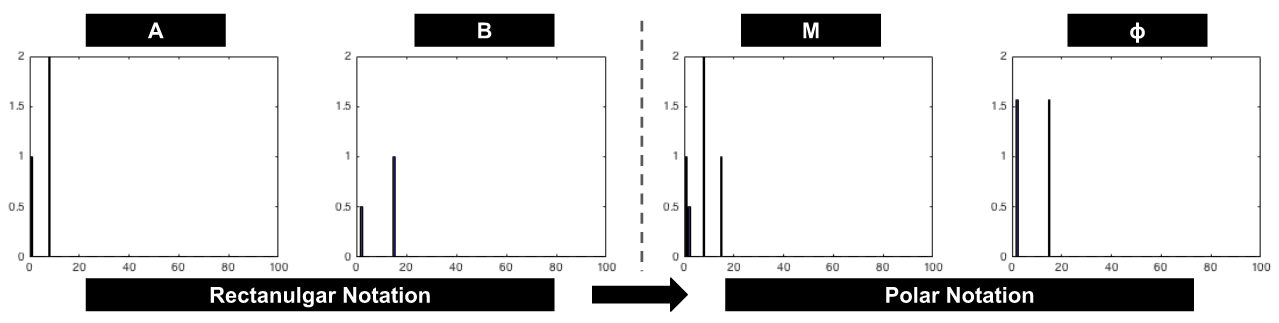
\includegraphics[width=1\textwidth]{bilder/rectToPolar02.png}
	\caption{Frequenz-Bereich des Beispiels aus Abbildung \ref{img:fftExample02}}
	\label{img:polarToRect02}
\end{figure}

Abbildung \ref{img:dtOverview} gibt einen Überblick über den Zusammenhang $x$ und $X$. Da mit steigender Länge von $x$ die Anzahl an Basis-Funktionen im Frequenzbereich $X$ steigt, wird die Auflösung des Frequenz-Bereiches umso höher, je länger $x$ gewählt wird. Im Gegenzug sinkt die Auflösung in Bezug auf den Zeit-Bereich: Der Frequenz-Bereich trifft keine Aussage darüber \emph{wann} etwas passiert, sondern nur \emph{welche Frequenzen} daran beteiligt sind.\cite[S. 170]{dspGuide}

\begin{figure}[h]
	\centering
	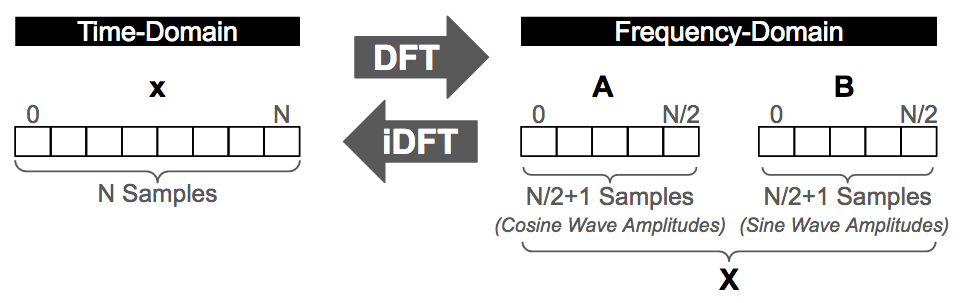
\includegraphics[width=0.8\textwidth]{bilder/dftOverview.png}
	\caption{Überblick über die DFT und die inverse DFT}
	\label{img:dtOverview}
\end{figure}


Aus Formel \ref{eq:inverseDFT} geht hervor, dass bei der Synthese jeweils ein Cosinus-Signal und ein Sinus-Signal der selben Frequenz addiert wird. Diese Addition erzeugt einen sogenannten \emph{Sinusoiden}, eine Cosinuswelle mit der Amplitude $M$ der Phasenverschiebung $\phi$ nach Formel \ref{eq:sinusoid}.\cite[S. 162]{dspGuide}

\begin{equation}
\begin{split}
A \cos(x) + B \sin(x) = M \cos(x + \phi) \\
,M = \sqrt{A^2 + B^2} \;, \phi = arctan(B/A)
\end{split}
\label{eq:sinusoid}
\end{equation}

Auf Basis von Formel \ref{eq:sinusoid} lässt sich der gesamte Frequenz-Bereich in kartesischer Notation als Menge von Sinusoiden-Schwingungen mit den Magnituden $M_0 \ldots M_{N/2}$ und den Phasenverschiebungen $\phi_0 \ldots \phi_{N/2}$ ausdrücken. Formel \ref{eq:rectToPolar} definierte diese Transformation von kartesischer Notation in die \emph{polare Notation}. Formel \label{eq:polarToRect} definiert die dazu inverse Transformation. \cite[S. 162]{dspGuide} Abbildung \ref{img:polarToRect02} zeigt den Frequenzbereich in polarer Notation für das Beispiel aus  Abbildung \ref{img:fftExample02}.

\begin{equation}
\begin{split}
M_k = \sqrt{(A_k^2 + B_k^2 ) }\\
\phi_k= \arctan{(B / A) }
\end{split}
\label{eq:rectToPolar}
\end{equation}

\begin{equation}
\begin{split}
A_k= M_k \cdot \cos(\phi_k)\\
B_k = M_k \cdot \sin(\phi_k)
\end{split}
\label{eq:polarToRect}
\end{equation}

Die kartesische Notation wird verwendet, um die DFT und die inverse DFT zu berechnen. Die polare Notation hat den Vorteil, dass vor allem die Magnituden $M$ für den Menschen leichter zu interpretieren sind. Die Magnituden $M$ sind Audioingenieuren als \emph{Spectrum} bekannt und werden in dieser Arbeit auch als solches bezeichnet. Die Transformation in die polare Notation wird deshalb vor allem dann Angewandt, wenn der Mensch den Frequenz-Bereich interpretieren soll. \cite[S. 164]{dspGuide}

Ein Schlussbemerkung: In der Einleitung dieses Kapitels wurde erwähnt, dass die DFT \emph{zeit-diskrete, periodische, unendliche} Signale transformiert, während in der hier vorgestellten Erläuterung das Signal sowohl als endlich angenommen, als auch keine Aussage über die Periodizität gemacht wurde. Bei der DFT wird davon ausgegangen, dass das Signal \emph{außerhalb} des Supportes von $x$ unendlich oft wiederholt wird, um die Vorraussetzungen zu erfüllen. Dabei handelt es sich jedoch um einen \glqq matehmatischen Trick \grqq{} der nur in Ausnahmefällen Einfluss auf den Frequenz-Bereich hat. Diese Ausnahmefälle tangieren diese Arbeit jedoch nicht, weshalb sie an dieser Stelle nicht weiter erläutert werden.\cite[S. 145]{dspGuide}

\subsection{Komplexe DFT}
\label{sec:comDFT}

Gleichwohl die in Kapitel \ref{sec:realDFT} vorgestellte \emph{reelle DFT} hilft beim Verständnis des Frequenz-Bereiches hilft, ist die Berrechnung der DFT nach Formel \ref{eq:forwardDFT} Rechnerisch zu ineffizient, um in Echtzeit durchgeführt zu werden. Der am weitesten verbreitete Algorithmus zur Berechnung des Frequenz-Bereiches, die \emph{Fast Fouerier-Transformation} erlaubt hingegen die Berechnung der DFT in Echtzeit. Da die FFT auf der \emph{complexen} Variante der DFT basiert, wird sie an dieser Stelle vorgestellt. 

Die Basis der komplexen DFT ist die \emph{Eulerformel}, definiert in Formel \ref{eq:eulersRelation}. Sie erlaubt die Darstellung des Funktions-Werte einer Cosinus-Welle und einer Sinus-Welle der selben Frequenz und Amplitude als den Real/Imaginärteil eines komplexen Exponenten der Eulerschen Zahl $e$. Gleichung \ref{eq:eulersRelationDetailed} zeigt, dass die Isolierung des Real/Imaginärteil von $e^{ix}$ Zugriff auf Funktionswert der entsprechenden Cosinus/Sinuswelle erlaubt. Auf einen Beweis der Eulergleichung wird an dieser Stelle aus Platzgründen verzichtet. Abbildung \ref{img:eulersRelation} visualisiert diesen Zusammenhang.

\begin{equation}
e^{ix} = \cos(x) + i\sin(x)
\label{eq:eulersRelation}
\end{equation}

\begin{equation}
\begin{split}
\Re(e^{ix}) = \cos(x) \\
\Im(e^{ix}) = \sin(x) 
\end{split}
\label{eq:eulersRelationDetailed}
\end{equation}

\begin{figure}[h]
	\centering
	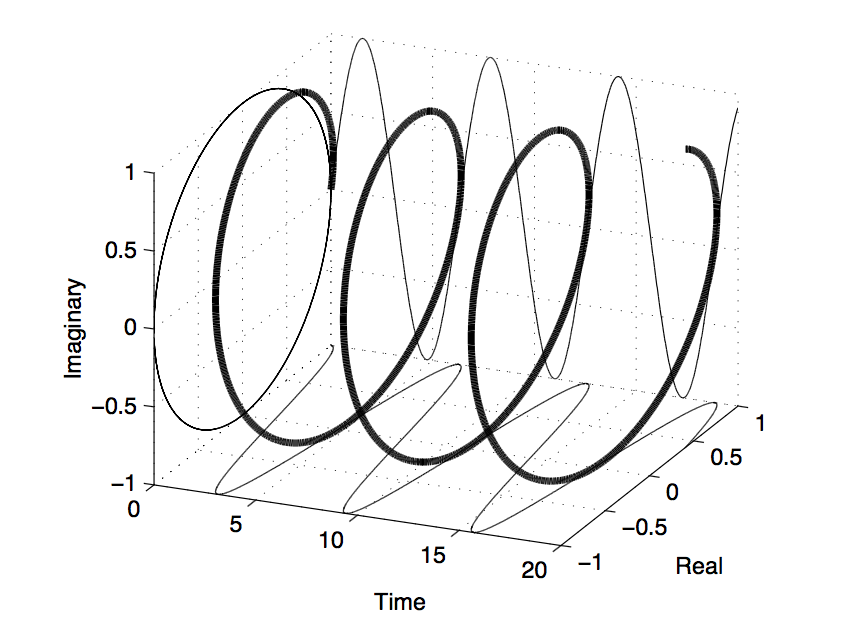
\includegraphics[width=0.5\textwidth]{bilder/eulersRelation.png}
	\caption{Visualisierung der Eulergleichung. Es wurde eine zuästzliche Zeit-Achse eingeführt, welche den Wert von $x$ als Funktionswert der Zeit darstellt\cite[S. 63]{dspMichigan}}
	\label{img:eulersRelation}
\end{figure}

Dementsprechend lassen sich die Basisfunktionen aus Gleichung \ref{eq:baseFunctions} ebenfalls durch den Real/Imaginärteil der von $e^{ix}$ nach Gleichung \ref{eq:complexBaseFunktion} definieren. Sie werden als die \emph{komplexe Basisfunktionen} bezeichnet. Die Frequenz der jeweiligen Basisfunktion wird, wie in Formel \ref{eq:baseToFreq} definiert, durch  $f = k\frac{f_s}{N}$ errechnet. 

\begin{equation}
\begin{gathered}
\Re(e^{i\cdot 2\pi k \frac{n}{N}}) = \cos_k[n] = \cos(2\pi k \frac{n}{N}) \\
\Im(e^{i\cdot 2\pi k \frac{n}{N}}) = \sin_k[n] = \sin(2\pi k \frac{n}{N})
\end{gathered}
\label{eq:complexBaseFunktion}
\end{equation}

Auf Basis dieses Zusammenhanges wird die \emph{komplexe DFT} in \emph{kartesischer Notation} nach Formel \ref{eq:complexDFTrectanulgar} definiert, das heißt die Transformation vom Zeit-Bereich in den Frequenzbereich mit Hilfe komplexer Zahlen. Formel \ref{eq:complexDFTpolar} definiert die komplexe DFT in der kompakteren, \emph{polaren Notation}.

\begin{equation}
\label{eq:complexDFTrectanulgar}
X[k] = \frac{1}{N} \sum_{n = 0}^{N-1}  x[n] \cdot (\cos (2\pi k \frac{n}{N}) -i \sin (2 \pi k \frac{n}{N}) )
\end{equation}

\begin{equation}
\label{eq:complexDFTpolar}
X[k] =  \frac{1}{N} \sum_{n = 0}^{N-1}  x[n] \cdot e^{-i 2\pi k \frac{n}{N}}
\end{equation}

Die wichtigen Unterschiede zwischen den komplexen DFT nach Formel  \ref{eq:complexDFTrectanulgar} und der reellen DFT nach Formel \ref{eq:forwardDFT} Formelsind (a) die Verwendung des Sinus als komplexe Zahl $i \cdot \sin$, sowie das invertieren seines Vorzeichens und (b) die Summierung über $n = 0\ldots N-1 $ anstatt $n = 0 \ldots N/2$. Der Frequenz-Bereich wird nun durch das complexe Signal $X$ ausgedrückt, welcher die Koeffizienten $A,B$ in seinem Real/Imaginärteil speichert. Der Frequenz-Bereich $X$ hat die selbe Länge wie der Zeit-Bereich $x$, das heißt $\text{Duration}(x) = \text{Duration}(X)$ Es gelten die die folgenden Zusammenhänge zwischen der reellen und der komplexen DFT \ref{eq:relationOfRealAndComplexDFT}. Es lässt sich ableiten, dass für die Indexe $k = 0 \ldots N/2$ die Real/Imaginärteil der komplexen DFT $X$ den Koeffizienten $A,B$ der reellen DFT entspricht. Da $|X| = M$, wird in dieser Arbeit $X$ ebenfalls als \emph{Spetrum} bezeichnet. 

\begin{equation}
\begin{gathered}
\Re(X[0]) \ldots \Re(X[N/2]) = A_0 \ldots A_{N/2} \\
\Im(X[0]) \ldots \Im(X[N/2]) = B_0 \ldots B_{N/2}  \\
|(X[0])| \ldots |(X[N/2])| = M_0 \ldots M_{N/2} \\
\phi((X[0])) \ldots \phi(X[N/2]) = \phi_0 \ldots \phi_{N/2} 
\end{gathered}
\label{eq:relationOfRealAndComplexDFT}
\end{equation}

Die \emph{inverse komplexe DFT} kann, genau wie die komplexe DFT, sowohl in polarer als auch in kartesischer Notation definiert werden. Gleichung \ref{eq:inverseComplexDFTpolar} definiert die iDFT in polarer Notation und Gleichung \ref{eq:inverseComplexDFTrectangular} in kartesischer Notation. Die polare Notation ist kompakter und die Variante, in der die komplexe inverse DFT meistens angegeben wird. Die kartesische Notation hingegen erleichtert das Verständnis. 

\begin{equation}
\label{eq:inverseComplexDFTpolar}
x[n] =  \sum_{k = 0}^{N-1}  X[n] \cdot e^{i 2\pi k \frac{n}{N}}
\end{equation}

\begin{equation}
\begin{split}
x[n] =  \sum_{k = 0}^{N-1}  
\Re(X[n]) \cdot (\cos (2\pi k \frac{n}{N}) + i \sin (2 \pi k \frac{n}{N}) ) \\ 
- \sum_{k = 0}^{N-1}
\Im(X[n]) \cdot (\sin (2\pi k \frac{n}{N}) - i \cos(2 \pi k \frac{n}{N}) )
\end{split}
\label{eq:inverseComplexDFTrectangular}
\end{equation}

Die Frage ist: Wenn das Signal des Zeit-Bereiches$x$  aus reellen Zahlen besteht, und das Signal des Frequenz-Bereiches $X$ aus komplexen Zahlen, wie \glqq verschwinden \glqq{} diese komplexen Zahlen wieder bei der Berechnung der inversen DFT? 

Genau wie das Signal des Zeitbereiches $x$ als unendlich und periodische außerhalb des transformierten Bereiches $x[0] \ldots x[N-1]$ angenommen wird, ist auch der Frequenz-Bereich unendlich periodisch außerhalb des Bereiches $X[0] \ldots X[N-1] $. Daraus lässt sich Schlussfolgern, dass $X[-N/2] \ldots X[-1] = X[N/2] ... X[N-1]$. Die Werte $X[-N/2] ... X[-1]$ werden als die \emph{negativen Frequenzen} bezeichnet. Dazu kommt der Fakt, dass der Frequenz-Bereich in Bezug auf das Interval $X[-N/2] \ldots X[N/2]$ eine Symmetrie aufweist: Der Realteil ist Achsensymmetrisch an der Stelle $X[0]$, und der Imaginäre Teil Punktsymmetrisch. Diese Symmetrie tritt nur auf, falls das Signal im Zeitbereich nur aus Reellen Zahlen besteht, was bei der Arbeit mit \glqq normalen Signalen\grqq{} immer erfüllt ist. Auf die Herleitung dieser Symmetrie wird an dieser Stelle aus Platzgründen verzichtet. 


Abbildung 	\ref{img:complexDFTOverview} gibt einen Überblick über die Indexierung bei der komplexen DFT.

\begin{figure}[h]
	\centering
	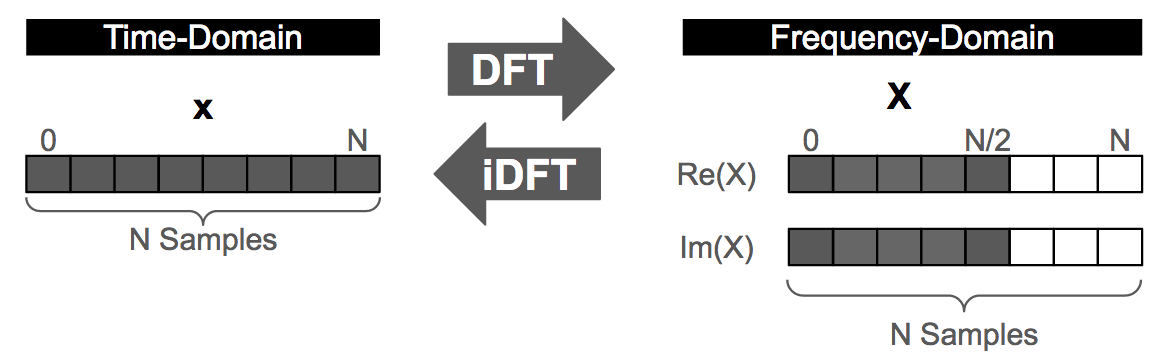
\includegraphics[width=0.8\textwidth]{bilder/compDFTOverview.png}
	\caption{Überblick über die komplexe DFT und inverse DFT}
	\label{img:complexDFTOverview}
\end{figure}


%Durch das Umformen der Eulergleichung lassen sich Cosinus- und Sinuswellen allein durch komplexe Exponenten von $e$ darstellen, zu sehen in Formel \ref{eq:complexSineCosine} .

%\begin{equation}
%\begin{gathered}
%\cos(x) = \frac{e^{ix} + e^{-ix}}{2} = \frac{1}{2} e^{-ix} + \frac{1}{2} e^{ix} \\
%\sin(x) = \frac{e^{ix} - e^{-ix}}{2i} = \frac{1}{2} ie^{-ix} - \frac{1}{2} ie^{ix}
%\end{gathered}
%\label{eq:complexSineCosine}
%\end{equation}

\section{Filter}
\label{sec:filter}

\section{akustische Modellierung der menschlichen Stimme}
\section{Feststellung von Periodizität in Signalen}
\subsection{Zero-Crossing-Rate}
\subsection{Methoden des Frequenzbereiches}
\subsection{Autokorrelation}
\subsection{Cepstrum}